% !TEX TS-program = pdflatex
% !TEX encoding = UTF-8 Unicode

% This is a simple template for a LaTeX document using the "article" class.
% See "book", "report", "letter" for other types of document.

\documentclass[11pt]{article} % use larger type; default would be 10pt


\usepackage{ulem}
\newcommand\NoIndent[1]{%
  \par\vbox{\parbox[t]{\linewidth}{#1}}%
}


\usepackage[utf8]{inputenc} % set input encoding (not needed with XeLaTeX)

%%% Examples of Article customizations
% These packages are optional, depending whether you want the features they provide.
% See the LaTeX Companion or other references for full information.

%%% PAGE DIMENSIONS
\usepackage{geometry} % to change the page dimensions
\geometry{a4paper} % or letterpaper (US) or a5paper or....
% \geometry{margin=2in} % for example, change the margins to 2 inches all round
% \geometry{landscape} % set up the page for landscape
%   read geometry.pdf for detailed page layout information

\usepackage{graphicx} % support the \includegraphics command and options

% \usepackage[parfill]{parskip} % Activate to begin paragraphs with an empty line rather than an indent

%%% PACKAGES
\usepackage{booktabs} % for much better looking tables
\usepackage{array} % for better arrays (eg matrices) in maths
\usepackage{paralist} % very flexible & customisable lists (eg. enumerate/itemize, etc.)
\usepackage{verbatim} % adds environment for commenting out blocks of text & for better verbatim
\usepackage{subfig} % make it possible to include more than one captioned figure/table in a single float
% These packages are all incorporated in the memoir class to one degree or another...

%%% HEADERS & FOOTERS
\usepackage{fancyhdr} % This should be set AFTER setting up the page geometry
\pagestyle{fancy} % options: empty , plain , fancy
\renewcommand{\headrulewidth}{0pt} % customise the layout...
\lhead{}\chead{}\rhead{}
\lfoot{}\cfoot{\thepage}\rfoot{}

%%% SECTION TITLE APPEARANCE
\usepackage{sectsty}
\allsectionsfont{\sffamily\mdseries\upshape} % (See the fntguide.pdf for font help)
% (This matches ConTeXt defaults)

%%% ToC (table of contents) APPEARANCE
\usepackage[nottoc,notlof,notlot]{tocbibind} % Put the bibliography in the ToC
\usepackage[titles,subfigure]{tocloft} % Alter the style of the Table of Contents
\renewcommand{\cftsecfont}{\rmfamily\mdseries\upshape}
\renewcommand{\cftsecpagefont}{\rmfamily\mdseries\upshape} % No bold!

%%% END Article customizations


\usepackage{verbatim}
\usepackage{amsmath}


\title{Work Log for October}
\author{Logan Brown}
%\date{} % Activate to display a given date or no date (if empty),
         % otherwise the current date is printed 


\begin{document}
\maketitle
\tableofcontents

\newpage


\section{Goals for the Month}
%Paste output from writeGoals
\begin{enumerate}
\item Find out what causes some of the probabilties to go outrageously high
\item Use the Simulated Yeast Genome, compare to the Ecoli genome
\item If possible, NSE Patch
\item Debugging Thoughts
\end{enumerate}

\section{Progress/Notes}

\subsection{Find out what causes some of the probabilties to go outrageously high}

\subsubsection{Compare Differences in the Code}
\begin{verbatim}
my.coef.r
my.drawPhiConditionalAllPred.r
my.drawPhiConditionalAll.r
my.estimatePhiOne.r
my.fitMultinomOne.r
my.logdmultinomCodOne.r
my.objectivePhiOne.Lfp.r
my.objectivePhiOne.nlogL.r
my.objectivePhiOne.nlogphiL.r
my.objectivePhiOne.phiLfp.r
my.pPropTypeNoObs.lognormal_bias.r
plotbin.r
plotmodel.r
simu.orf.r
\end{verbatim}


Codes where NSE and ROC are the same:
\begin{enumerate}
\item my.coef.r
\item my.estimatePhiOne.r

\end{enumerate}


\subsection{Look at stddev(phi)}

I have a run going that is tracking the scales of the MCMC for the phi values.

Since the scale of the MCMC should be about the Standard Devation of Phi, we'll see what happens.

PROBLEM:
The ROC model has different Phi scales for each gene. The NSE model keeps all the scales the same between different genes. That could be contributing to the problem? \sout{I think this is caused by the opatch we wrote that replaces Wei-Chen's scaling by .5  with subtracting out log(DBL\_MAX).}

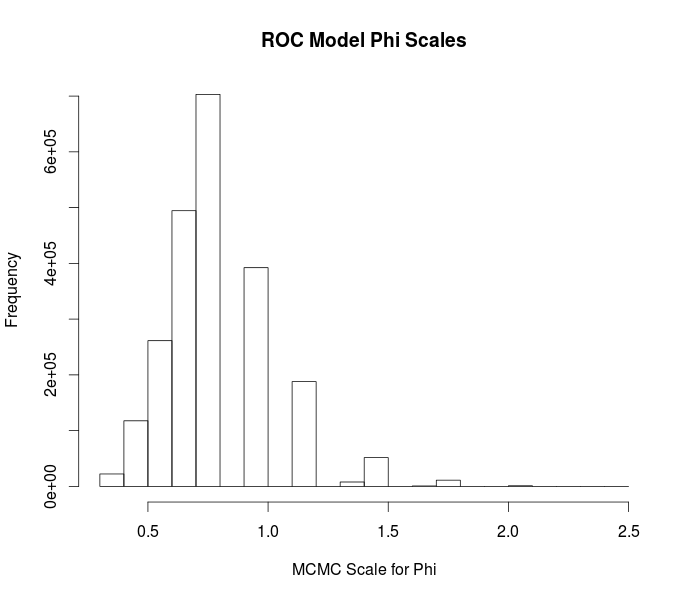
\includegraphics[width=0.5\textwidth]{data/oct10-roc-scalehist.png}
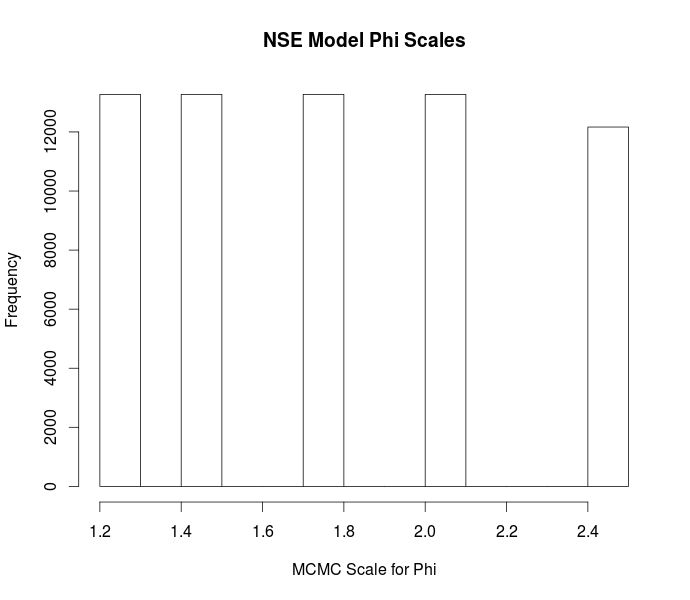
\includegraphics[width=0.5\textwidth]{data/oct10-nse-scalehist.png}

\textbf{Every 6th time that the scale is updated, the code resets all the scales to 1. This definitely happens in Yeast (NSE and ROC), and I think it happens in E Coli. Needs further testing.}


\subsection{Simulated Yeast Genome}

\subsubsection{Use Sections of the Simulated Yeast Genome}
I ran one 5th of the yeast genome(section1.fasta, section1.csv) and it FINISHED. but... not well.

See the results in data/10.01.yeastnse.*

\begin{itemize}
\item It took just over 30 hours to finish\\
started at: 2014-10-01 15:57:54\\
finished at: 2014-10-02 22:08:56 

\item The proposed phi values are still outrageously too high. The final proposed phi had mean value 2766786.09545948

\item Still proposing some 0 (-Inf) values for lpProp. At most, around 45-49 Inf per run.

\item Xobs (the original phi values) are generally much lower than the results of run

\item The values are not very accurate.

\end{itemize}


\subsubsection{Crashed Yeast Run}

The vast vast majority of the phi values being proposed are fine. -Inf values are throwing it off. 


\subsection{E. Coli genome}

A LARGE NSE RUN OF THE E. COLI GENOME RAN TO COMPLETION.



\subsection{If possible, NSE Patch}






\section{Goals for next Month}
\begin{enumerate}
\item Future Goal
\end{enumerate}


\end{document} %End of day document, REMOVE
